<<<<<<< HEAD
\section{Procedure}
\label{sec:procedure}

A \emph{Geodreieck} is used.

\begin{figure}
	\label{fig:geodreieck}
	\centering
	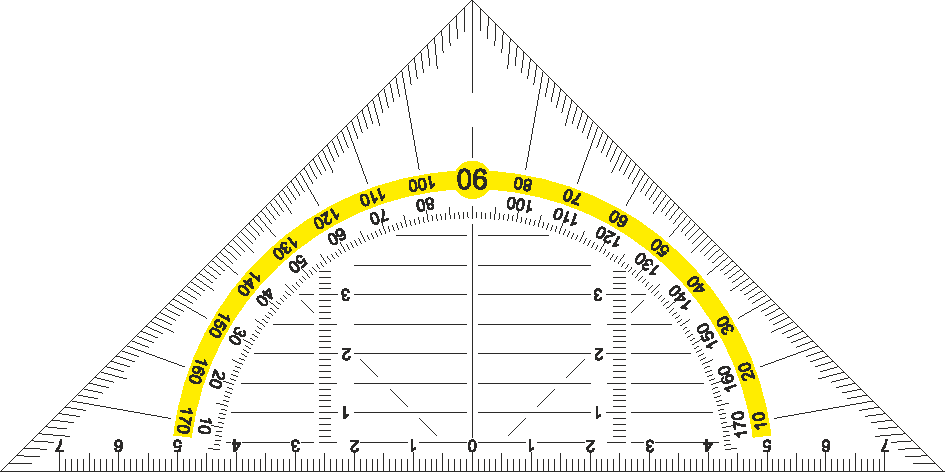
\includegraphics[width=0.55\textwidth]{content/graphics/geodreieck.pdf}
	\caption{Schematic depiction of a \emph{Geodreieck}.}
\end{figure}
||||||| 4f7bc50
=======
\section{Procedure}

\subsection{Aligning the laser}

\subsection{Verifying the stability condition}

\subsection{Observing transverse modes}

\subsection{Determining the polarization}

\subsection{Analyzing spectra in multimode operation}

\subsection{Measuring the wavelength}
>>>>>>> 9d01d58a6b381b59ed11432e8164b119046f2cb6
